% latex article template

% cheat sheet(eng): http://www.pvv.ntnu.no/~walle/latex/dokumentasjon/latexsheet.pdf
% cheat sheet2(eng): http://www.pvv.ntnu.no/~walle/latex/dokumentasjon/LaTeX-cheat-sheet.pdf
% reference manual(eng): http://ctan.uib.no/info/latex2e-help-texinfo/latex2e.html

% The document class defines the type of document. Presentation, article, letter, etc. 
\documentclass[12pt, a4paper]{article}

% packages to be used. needed to use images and such things. 
\usepackage[pdfborder=0 0 0]{hyperref}
\usepackage[utf8]{inputenc}
\usepackage[english]{babel}
\usepackage{graphicx}
\PassOptionsToPackage{hyphens}{url}

% hides the section numbering. 
\setcounter{secnumdepth}{-1}

% Graphics/image lications and extensions. 
\DeclareGraphicsExtensions{.pdf, .png, .jpg, .jpeg}
\graphicspath{{./images/}}

% Title or header for the document. 
\title{TDT4300 Datavarehus og datagruvedrift - Spring 2013 \\ Assignment 5: Cluster Validation}
% Author
\author{
        Magnus L Kirø \\
}
\date{\today}

\begin{document}
\maketitle
\pagenumbering{arabic}

\section{Evaluation}
From the graph in figure 2 \ref{fig:2} we can see the SSE value for the first
file. We clearly see that the error drops significantly at k=3 (the x-axis
represents k-1). This indicates that a clustering with three centroids give a
good clustering of the data in the data set. Similarly we can see in figure 6 
\ref{fig:6} that the best results are provided at k=2. The lower the SSE value
the better the clustering is. With fewer clusters we get faster computation
time, which is positive. Thus a lower value of k will give quicker results.
Althought maybe not the best results. 

SSE measures the cohesion of a cluster, og the entire dataset. This differs
from SSB which measures the independence of each cluster.
The silhouette value is a combination of SSB and SSE. 

The measures show the correctness of the clustering and what degree of
clustering should be used in this case. 

\section{Graphs and tables}
The two files are: "iris.arff" and "segment-challenge.arff".
Graph descriptions are in the image caption.
The x axis represents K-1.
% imgae example. 
\begin{figure}[htb]
    \centering
    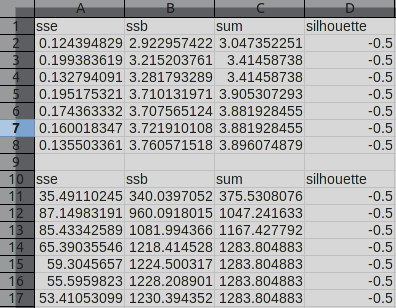
\includegraphics[width=\textwidth]{table}        
    \caption{Table containing all results from the two files. The top one is
the first file.}
    \label{fig:1}
\end{figure}


\begin{figure}[htb]
    \centering
    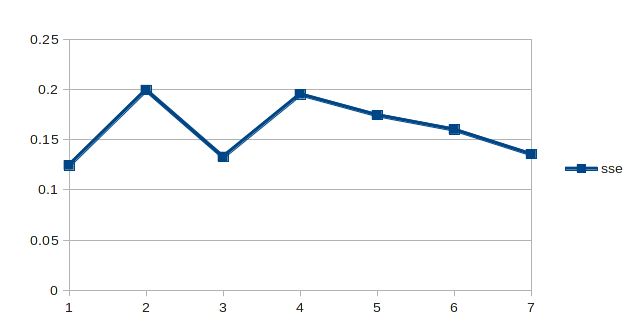
\includegraphics[width=\textwidth]{sse1} 
    \caption{SSE for the first file.}
    \label{fig:2}
\end{figure}

\begin{figure}[htb]
    \centering
    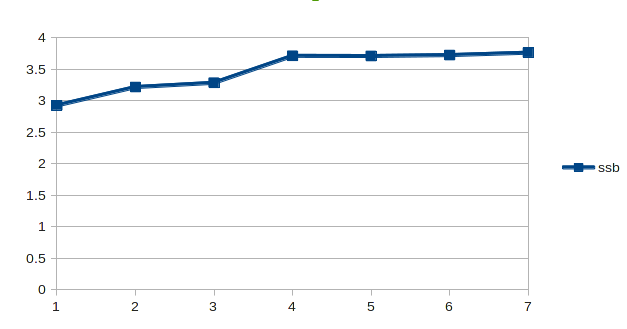
\includegraphics[width=\textwidth]{ssb1}
    \caption{Ssb for the first file.}
    \label{fig:3}
\end{figure}

\begin{figure}[htb]
    \centering
    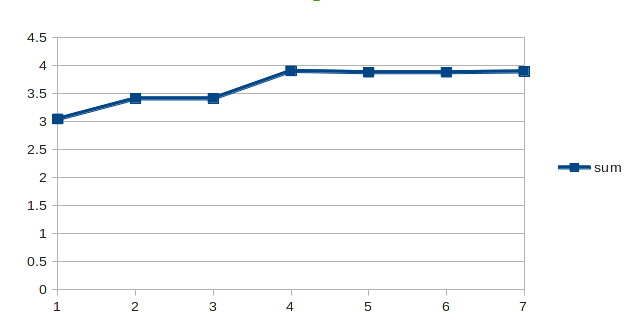
\includegraphics[width=\textwidth]{sum1}
    \caption{Sum for the first file.}
    \label{fig:4}
\end{figure}

\begin{figure}[htb]
    \centering
    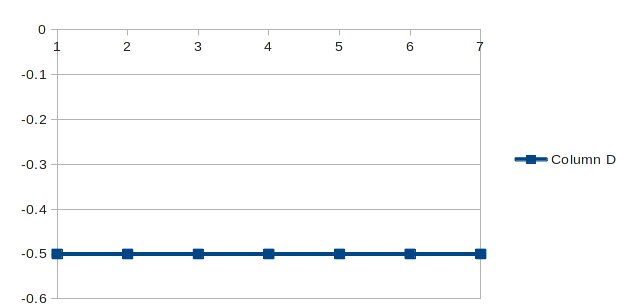
\includegraphics[width=\textwidth]{silhouette1}
    \caption{Shows the silhouette values for bot files. They were the same
consistently. There are probably some error in the code but I could not find
it.}
    \label{fig:5}
\end{figure}

\begin{figure}[htb]
    \centering
    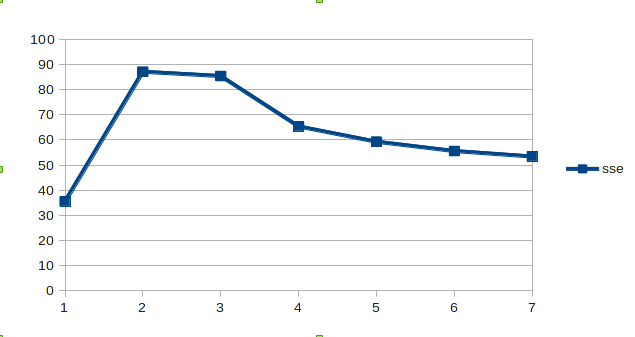
\includegraphics[width=\textwidth]{sse2}
    \caption{Shows the sse values for the second file}
    \label{fig:6}
\end{figure}

\begin{figure}[htb]
    \centering
    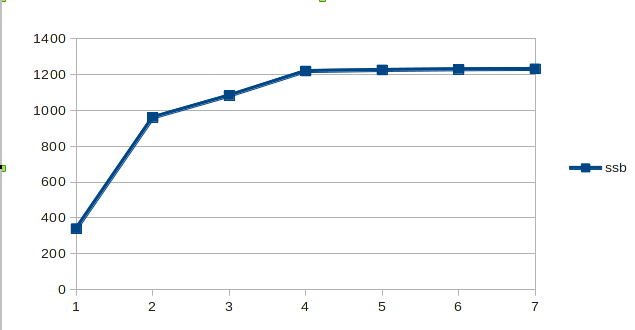
\includegraphics[width=\textwidth]{ssb2}
    \caption{Shows the ssb values for the second file.}
    \label{fig:7}
\end{figure}

\begin{figure}[htb]
    \centering
    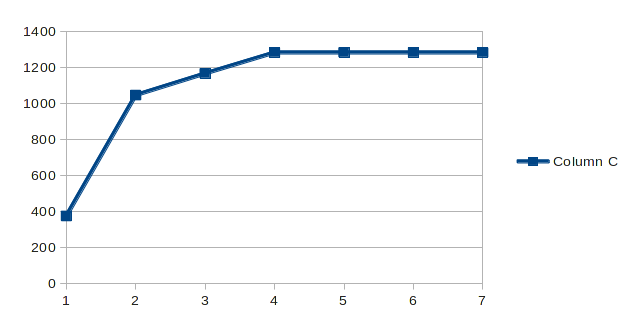
\includegraphics[width=\textwidth]{sum2}
    \caption{Shows the sum of the scond file.}
    \label{fig:8}
\end{figure}

\end{document}
